%!TEX root = ../main.tex

\section{CAN bus}\label{sec:CANbus}
The can is described in this section, starting with the implementation of the physical layer.

\subsection{Physical Layer}\label{sub:CANphys}
The physical layer has three main parts: The CAN controller, the CAN transceiver and the bus itself. \\

The Zybo supports CAN, and has a CAN controller in its PS.
An IP core is also available if FPGA implementation was desired.\\

The CAN transceiver is connected to the controller by Rx and Tx voltage signals, and connects to the bus through two differential ports. 
The transceiver must support the standard ISO11898-2, as this is what the Sevcon motor driver uses.
The device SN65HVD232 from Texas instruments support this standard, and is supplied with 3.3 V, so it can be plugged right into the Zybo, and still communicate with the Sevcon even though its CAN bus uses $\si{5 \volt}$.
According to TI itself\cite{3.3V_CAN}, this family of $\si{3.3 \volt}$ transceivers are compatible and interoparable with other \si{5 \volt} transceivers, so long as they support the same standard.\\

The transceivers have been mounted on boards, that plug directly into the Zybo's 12-pin PMOD connector, which will be stacked on top of each other. 
The schematic is shown below.

\begin{figure}[h!]
	\centering
	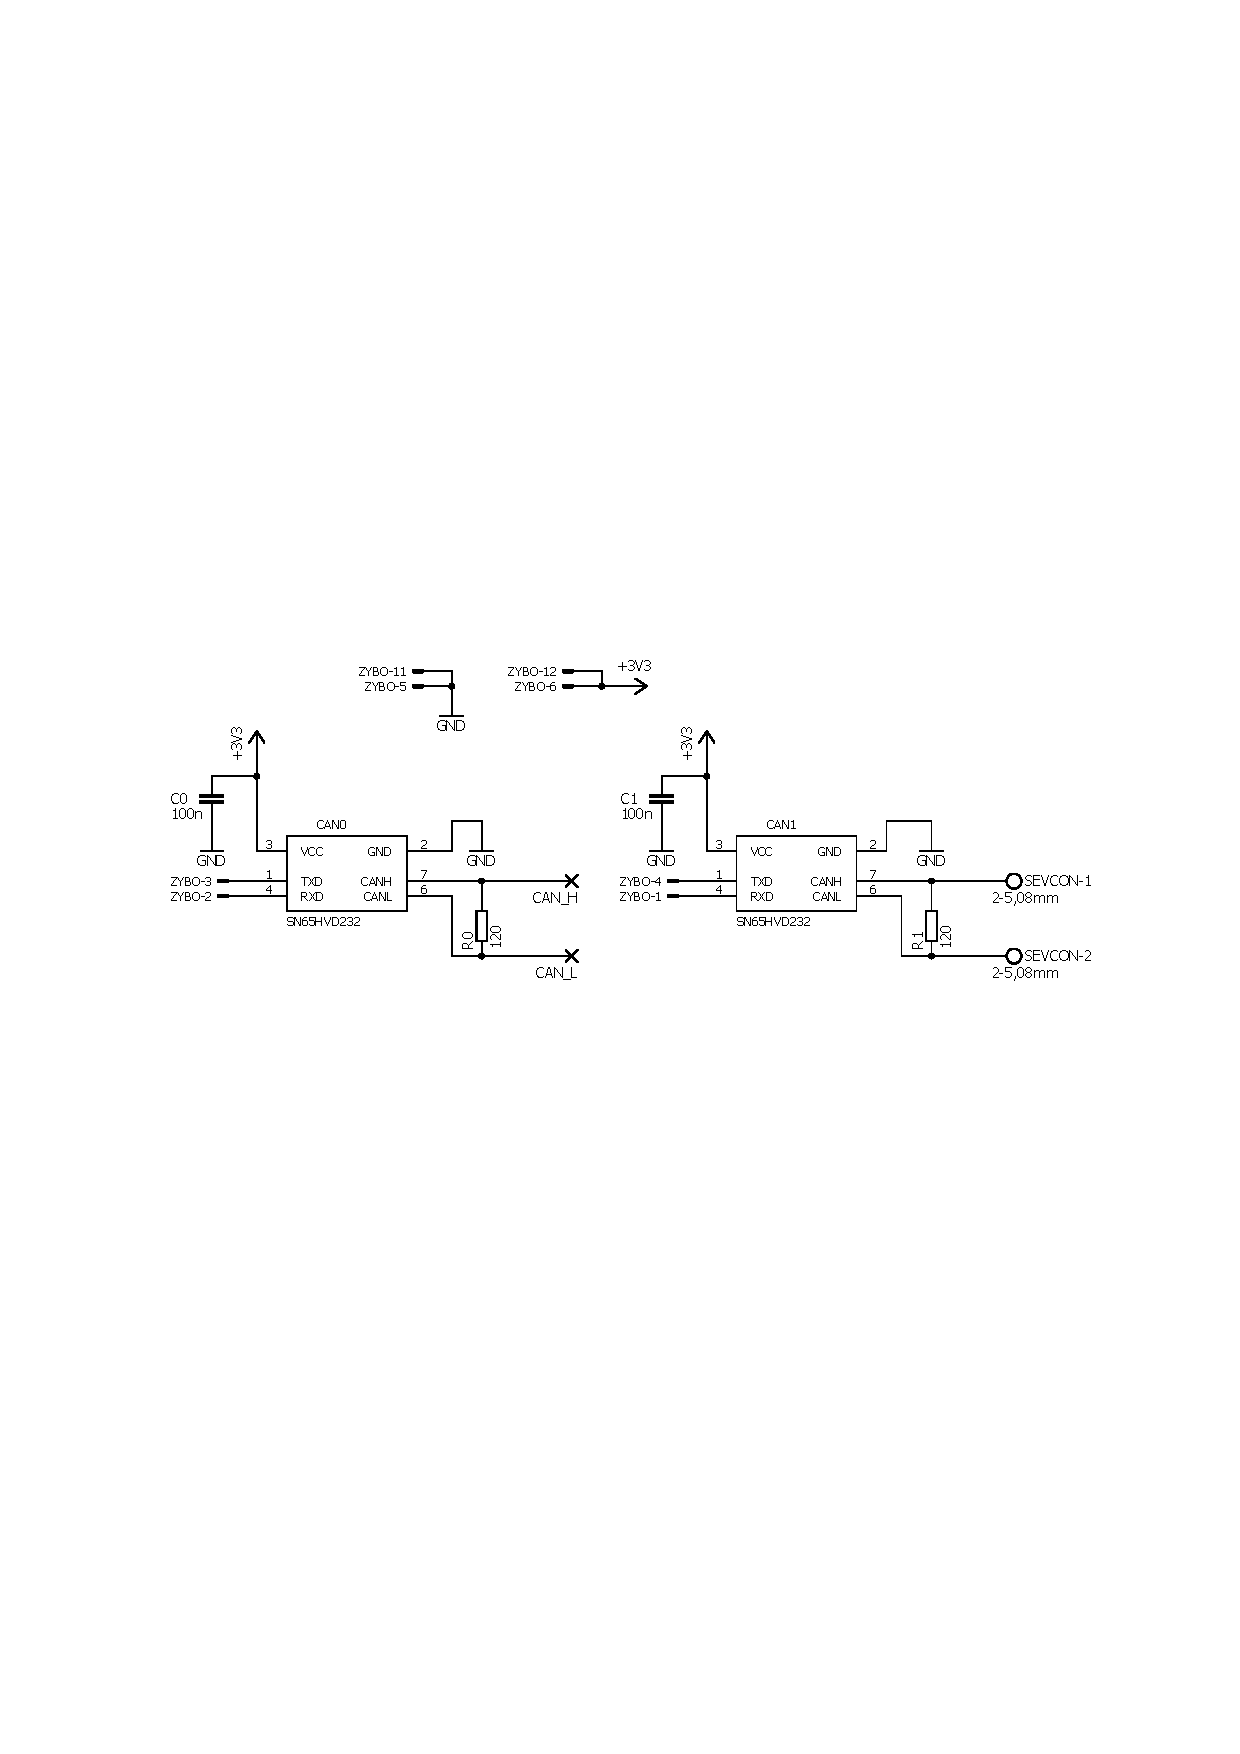
\includegraphics[width = 0.7\linewidth]{graphics/CAN_Schematic}
	\caption{Schematic of the two can transceivers. One board is build for two transceivers each with pads for termination}
	\label{fig:CAN_Schematic}
\end{figure}

The board has been designed to use the MIO ports, available in the PMOD JF. 
This is necessary to utilize the build in CAN controllers on the PS part of the Zybo.
Although the schematic contains two transceivers and two termination resistors, most of these devices are not mounted. 
Four boards will be made, all containing CAN0, C0 and the ZYBO connector. 
One board will also include the resistor R0 - this is the bottommost board
Another board will include R0, R1 CAN1, C1 and the SEVCON connector.
Ths is placed on top, to allow the SEVCON connector's screws to be accessible. 
The stack is visible below

\begin{figure}[H]
	\centering
	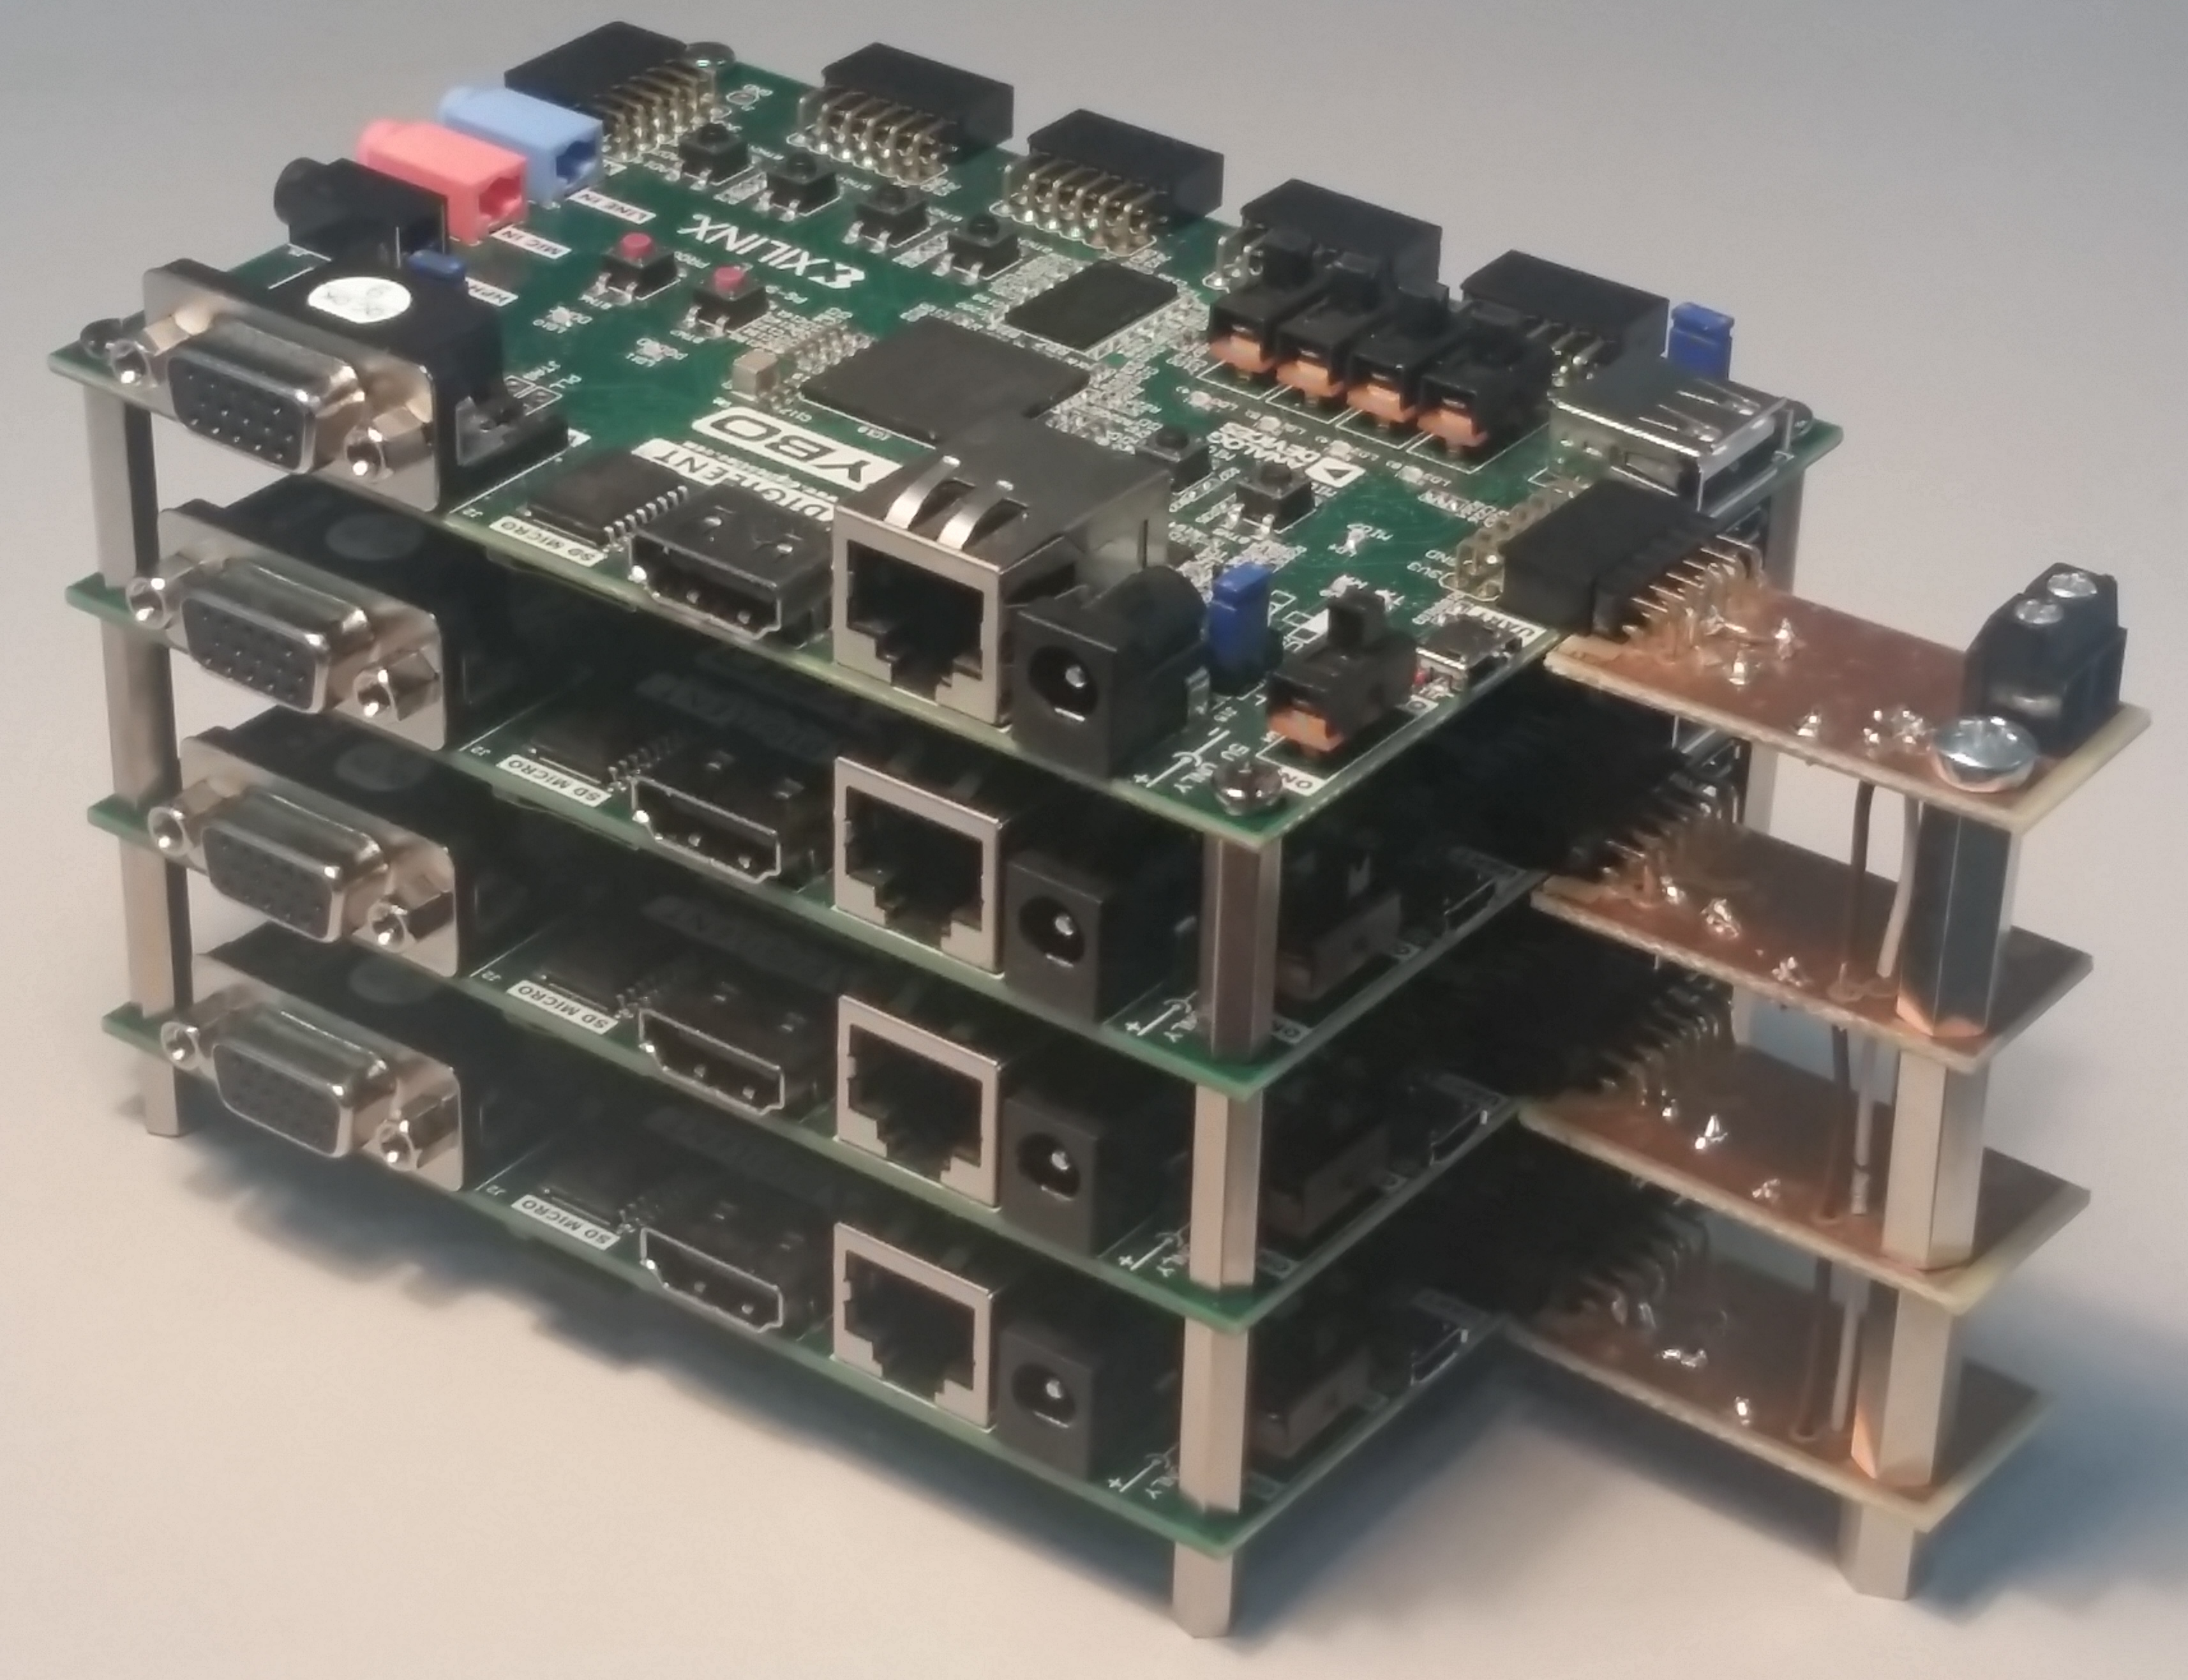
\includegraphics[width = 0.9\linewidth]{graphics/CAN_stack_picture}
	\caption{The CAN stack plugged into one Zybo}
	\label{fig:CAN_stack_picture}
\end{figure}

Because the bus is so short, it isn't practical to make twisted pair, and this will work fine.
The bus itself is also not $120 \si{\ohm}$, but experiment shows that it works.

\todo{Polish the text and re-express some things such as send() function...}
\subsection{Testing the CAN Stack for a Basic Network}
After the design and printing of the stack board, testing it was the next step.
The test included using one the CAN controllers within the Zynq chip with the purpose of showing that a basic CAN network between two Zybo boards could be implemented using the stack.
Specifically, the one Zybo was sending the input value of the buttons to the network in order to be received by the second one and turn on the on-board LEDs as a result.
After designing a basic architecture in Vivado and writing a source code, the test was successful, thus proving the basic functionality of a CAN network.
All Zybo boards were programmed with the same architecture and source code.

\subsubsection{Architecture}
In order to realize the above test, enabling the CAN controller inside the Zynq chip as well as including two AXI GPIO cores were necessary.
One AXI GPIO was setup as leds 4bits while the other one as btns 4bits as it can be seen in figure \ref{fig:CAN_Testing_Architecture}. The architecture was firmly simple, but adequate to meet the purpose of the test.

\begin{figure}[h!]
	\centering
	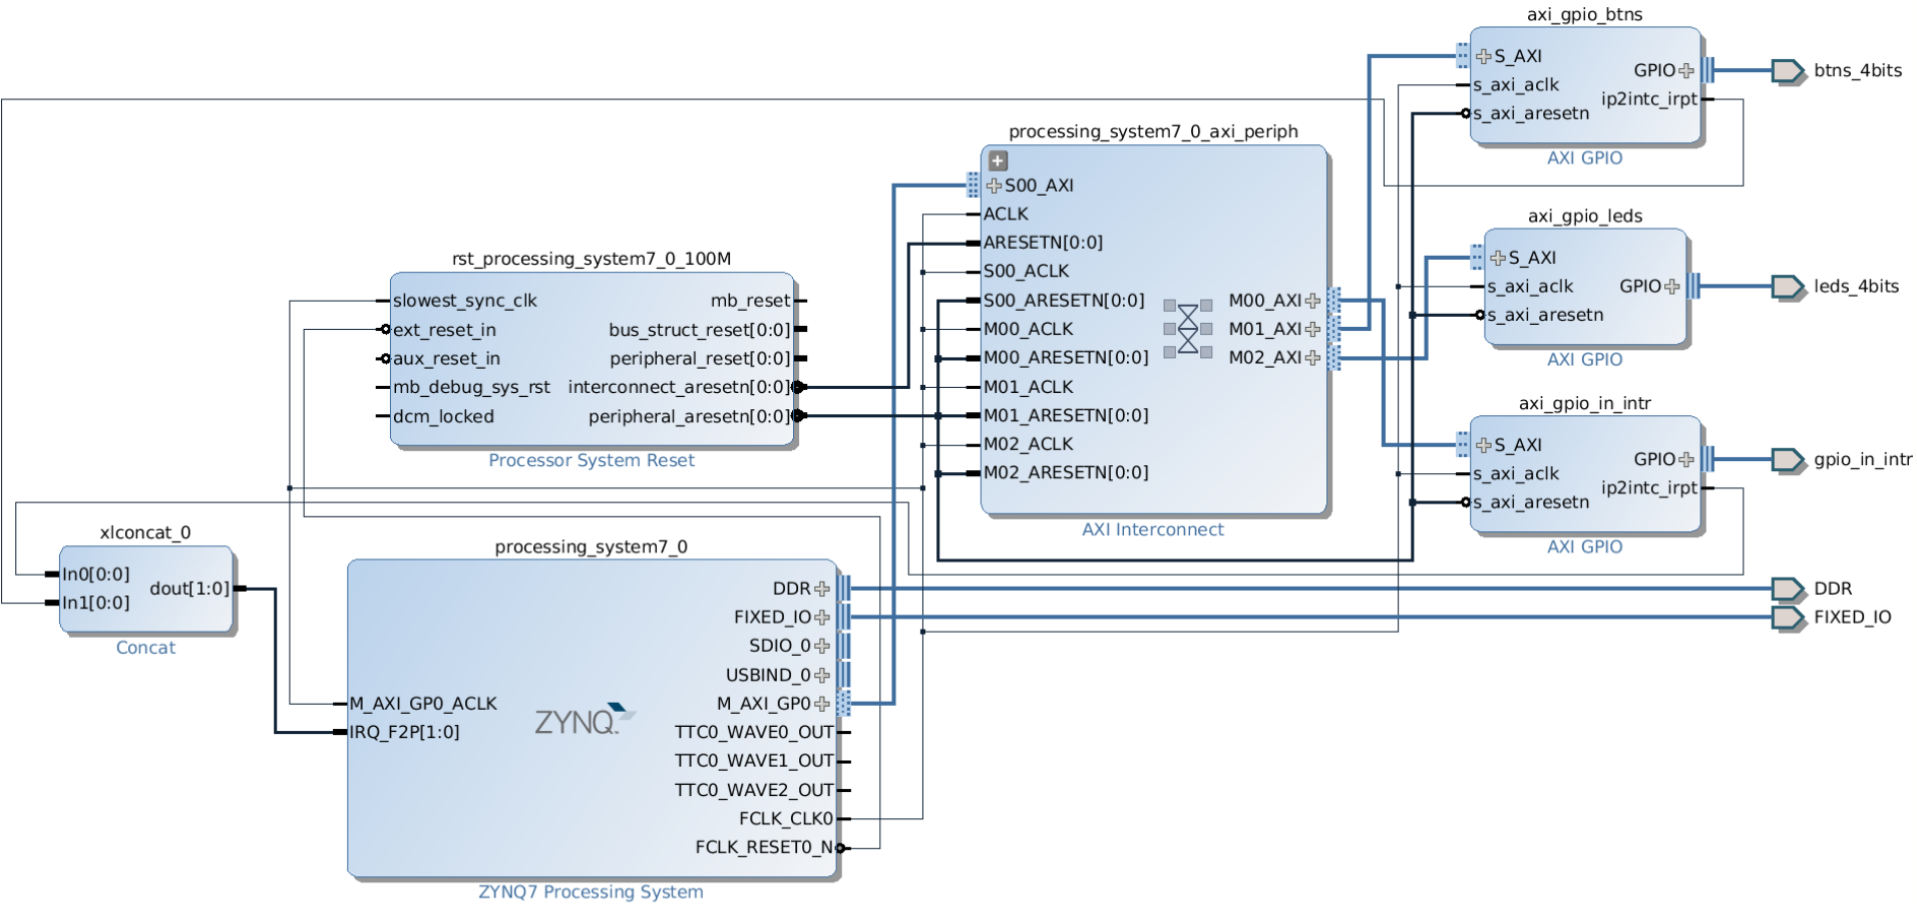
\includegraphics[width = 0.9\linewidth]{graphics/Zybo_BasicTestingArchitecture_for_CAN.png}
	\caption{Block diagram featuring the testing architecture in Vivado.}
	\label{fig:CAN_Testing_Architecture}
\end{figure}

\subsubsection{Source Code}
The programming for this task was done in C.
The code from xcanps polled example provided by Xilinx documentation was used as a basis.
The example shows the basic principle of sending and receiving messages on a loopback network on a single board.
With further modifications and the addition of extra functionalities such as reading button input and writing the output to the LEDs, the finalized developed code was suitable to test the communication between two nodes on the CAN network.
\\\\
The basic principle for testing was to trigger an interrupt attached to the button presses, which then the send() function would send the value of the buttons to the network as a message.
In turn, the receive() function was responsible of reading the message transmitted on the bus and writing the value as output to the LEDs.
As mentioned before, this source code was common and uploaded to both boards resulting in a two-way communication, since both of them had a send() and a receive() function, thus one controlling the LEDs of the other one.

\todo{We need a picture with 2 or better, 4 boards as stack! The coolest thing ever :P.}

\subsection{CAN Message Frame}\label{sub:CanMessageFrame}
Messages sent over CAN is put into a frame. 
One frame contains all the parts in figure~\ref{fig:CAN_frame_pdf}, whereas a message should not be restricted to just 8 bytes -- however it doesn't include any overhead.
A zero input to the transceiver will result in a voltage difference on the CAN bus, and a one input will result in no difference. 
A zero will alway be dominant -- this is used to ensure that two nodes to not talk at the same time.
If a node tries to write a one, but simultaneously reads back a zero, it will know that something is wrong, for instance, that the bus is occupied by a node with higher priority.
The CAN message consists 47 bits of overhead with each message of 0-8 bytes. 
This overhead includes a such things as message IDs and checks, to ensure that the message is received correctly, and collectively this is called a frame. 
The frame of the message is described here.

\begin{figure}[h!]
	\centering
	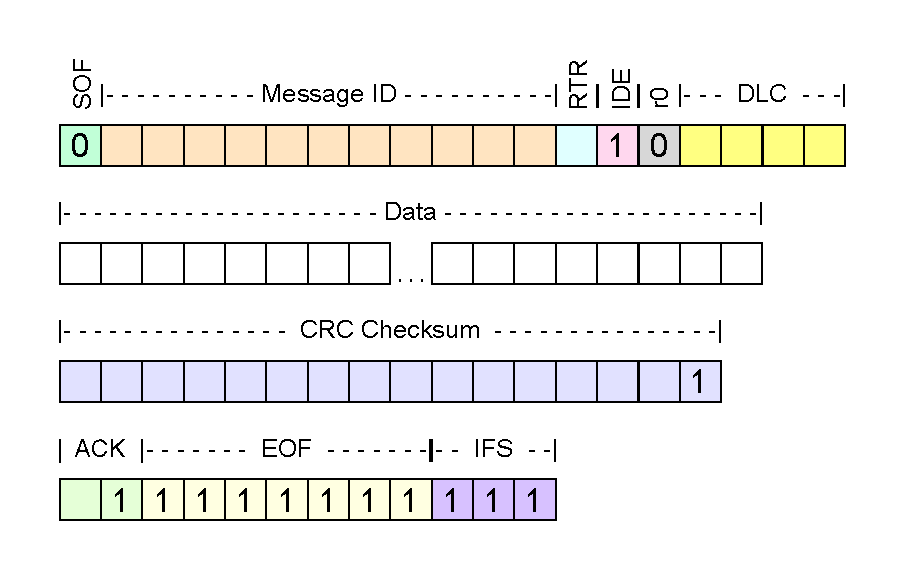
\includegraphics[width = 0.9\linewidth]{graphics/CAN_frame_pdf}
	\caption{Bitwise representation of a CAN frame}
	\label{fig:CAN_frame_pdf}
\end{figure}

\begin{itemize}
	\item SOF: \textbf{S}tart \textbf{O}f \textbf{F}rame: One dominant bit to start a frame.
	\item Message ID: 11 bit message identifier provides information about what the message contains. Subscribers will recognize a message by this ID.
	\item RTR: \textbf{R}emote \textbf{T}ransmission \textbf{R}equest: set to 1 if a transmission is requested from another node. Because is a publisher-subscriber network, this will always be 0.
	\item IDE: \textbf{ID E}xtended: Set to 1 if extended ID is in use. This adds 18 more bits of message identifiers immediately after this bit. At the moment, this is not needed, and should always be 0.
	\item r0: bit reserved for future use, alway set to zero
	\item DLC: \textbf{D}ata \textbf{L}ength \textbf{C}ode: how many bytes, of data, the frame contains. Ranging from 0-8.
	\item Data: Raw data. 
	\item CRC Checksum: \textbf{C}yclic \textbf{R}edundancy \textbf{C}heck: 15 bit checksum based on what was written in the Data portion. The last bit is a delimiter, and is always 1.
	\item ACK: \textbf{ACK}nowledge: The transmitting node will set the first bit of ACK to be recessive (1). Each receiving node will calculate CRC based on the data, and compare it to the CRC checksum. If no error is detected, it will set the bit to dominant (0). On a multi-node network, if one node confirms the data, the transmitting node cannot know if any other node did not receive the data. However, because of the nature of a differential voltage bus it is nearly impossible that two nodes would not receive the the same signal, so long as the bus is correctly impedance matched, and distances do not exceed the specification. The last bit o ACK is a delimiter, and always 1
	\item EOF: \textbf{E}nd \textbf{O}f \textbf{F}rame: Pattern signifies the end of a frame, the pattern is 7 recessive bits.
	\item IFS: \textbf{I}nter\textbf{F}rame \textbf{S}pace: an arbitrary length of recessive bits, at least three bits long. After this point, a new frame may start by setting a zero.
\end{itemize}

Because 0 dominates zero, it is possible to prioritize messages -- lower message ID get higher priority.
If two nodes start writing a message at the same time, the first node to write a 1 when the other node writes 0 will realize that another node has right of way, and will stop transmitting and wait for the current frame to end.
When the end of the message occurs, the node will try to send the message again.
It might then be blocked again by another node, and there is a risk, that it will never send.
It is the developer's responsibility to ensure that this doesn't happen.\\

It is, that messages are extended by bit stuffing.
If either 0 or 1 is written to the controller 5 consecutive times, the opposite polarity is interjected, or stuffed, into the stream. 
This is done to ensure that receiving nodes remain synchronized with the transmitting node, as there is no clock signal.
That means, that a frame can be extended by upwards of 20 \% if the data requires it.
